\chapter{Modellierung in der Architektur}
Der Architekturprozess \glqq erstreckt sich von der Analyse des Problembereichs eines Systems bis hin zu seiner Realisierung\grqq \cite[S. 10]{softarch} und arbeitet durch die verschiedenen Architektursichten stark mit verschiedenen Mitteln der Abstraktion. Wien in ISO 42010 beschrieben besitzt jede Architektursicht zudem ein oder mehrere Architekturmodelle \cite{ISO_ARCH}. Werden Architektursichten im Architekturprozess verwendet, bietet sich deswegen auch die Verwendung von Modellierungssprachen an, mit welchen die Architekturmodelle erstellt werden können.

\section{Modelldefinition}
Ein Modell hat laut Stachowiak folgende Eigenschaften \cite[S. 131-133]{modell}:

\begin{itemize}
  \item Abbildung
  \item Verkürzung
  \item Pragmatismus
\end{itemize}

Das Abbildungsmerkmal besagt, dass Modelle entweder natürliche oder künstliche Dinge abbilden. Das Verkürzungsmerkmal eines Modells dreht sich um die Reduktion der Eigenschaften des Originals: Nur die für den Einsatzbereich relevanten Eigenschaften werden durch das Modell repräsentiert. Das Pragmatismusmerkmal schließlich besagt, dass Modelle eine Funktion erfüllen: Sie sind sowohl für einen definierten Einsatzzweck, als auch für eine Person, sei sie natürlich oder künstlich, erstellt. \cite[S. 131-133]{modell}

Werden Modelle verwendet, müssen diese kommuniziert und dokumentiert werden \cite[S. 12]{reqanalysis}. Vor Allem in der Arbeit im Team bietet sich deswegen eine standardisierte Modellierungssprache an, welche den Einsatzbereich so gut wie möglich abdeckt. Dies dient vor Allem dazu, Interpretationsfehler zu vermeiden. Aus dem gleichen Grund ist es auch vorteilhaft, eine weit verbreitete Modellierungssprache zu wählen \cite[S. 139]{effektiv}. Eine Modellierungssprache sollte zudem visuelle Elemente verwenden, da das menschliche Auge Bilder schneller als Text aufnehmen kann \cite[S. 12]{reqanalysis}.

\section{UML}
UML, kurz für Unified Modelling Language, ist eine in den 90ern entstandene Modellierungssprache, welche sich vor Allem für die Modellierung objektorientierter Systeme eignet \cite[S. 145]{basiswissen}. Sie war eine Antwort auf den damaligen Wildwuchs an verschiedenen, zueinander inkompatiblen Modellierungssprachen wie OOD, OOA\&D, etc. \cite[S. 5]{glasklar}. Mittlerweile ist sie weit verbreitet und wird weltweit verstanden \cite[S. 138]{effektiv}. Die aktuelle Version der UML ist 2.4.1 \cite{omg}.


Die in der UML spezifizierten Diagramme lassen sich in folgende zwei Kategorien einteilen \cite[S. 105, 239]{glasklar}\cite[S. 146]{basiswissen}:

\begin{itemize}
  \item Verhaltensdiagramme
  \item Strukturdiagramme
\end{itemize}

UML Diagramme lassen sich im Architekturprozess vor Allem zur Beschreibung der verschiedenen Architektursichten einsetzen und bieten alle für die Abstraktion des Systems im Architekturprozesses benötigten Werkzeuge\cite[S. 139]{effektiv}. Durch ihre verkürzende Wirkung und höhere Informationsdichte sind UML Diagramme auch oft Artefakte des Anforderungsprozesses \cite[S. 215]{reqman}. UML schlägt somit die Brücke vom Anforderungs- zum Architekturprozess. Nicht alle verfügbaren UML Diagramme sind jedoch für die Erstellung und Modellierung der Architektur nötig. \cite[S. 144]{basiswissen}

Die in der Arbeit verwendeten Verhaltensdiagramme beschränken sich auf das Usecase-, Kontext-, Komponenten- und Aktivitätsdiagramm. Das einzig verwendete Strukturdiagramm ist das Klassendiagramm.


\subsection{Usecasediagramm}
Das Usecasediagramm gliedert sich in die Diagrammkategorie der Verhaltensmodellierung ein und beschreibt die Anwendungsfälle des Systems, dessen AkteurInnen und die Beziehung zwischen den Beiden. Die einzelnen Anwendungsfälle selbst repräsentieren Aktionen. Diese werden jedoch nicht im Usecasediagramm modelliert.\cite[S. 242-245]{glasklar}

\begin{figure}[H]
    \centering
    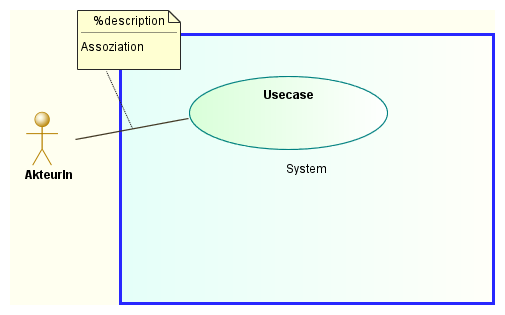
\includegraphics[scale=0.8]{uml/modelling/usecase.png}
    \caption{Das UML Usecasediagramm}
    \label{fig:umlusecasemodel}
\end{figure}

Das Usecasediagramm ist kein Artefakt der Architekturerstellung, sondern wird in der Regel in der Anforderungsanalyse des Projektes erstellt. In der Architekturphase gibt das Diagramm aber Auskunft über wichtige architekturentscheidende Parameter, wie zB. die Systemabgrenzung, Nachbarsysteme, Benutzer und Grundfunktionalität des Systems. Außerdem wird es für Architekturreviewmethoden wie ATAM benötigt und kommt in der Usecase Sicht von Kruchtens 4+1 Modell vor \cite[S. 148]{basiswissen}

\subsection{Kontextdiagramm}
Das Kontextdiagramm kann in die Strukturmodellierung eingeordnet werden und zeigt die AkteurInnen, Datenflüsse und Nachbarsysteme. Das Kontextdiagramm selbst ist nicht Teil der UML, kann aber mit UML dargestellt werden. Meistens wird dafür ein Usecasediagramm verwendet, aber auch ein Komponentendiagramm stellt im Prinzip die notwendigen Elemente bereit. \cite[S. 255]{glasklar}

\begin{figure}[H]
    \centering
    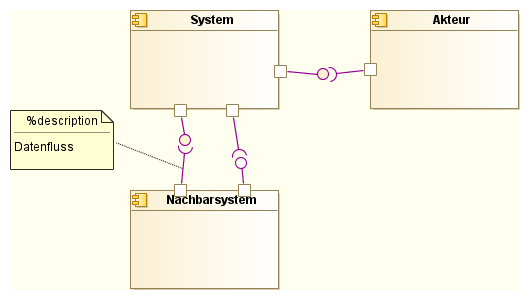
\includegraphics[scale=0.8]{uml/modelling/context.png}
    \caption{Das Kontextdiagramm, dargestellt mit Hilfe des Komponentendiagramms}
    \label{fig:umlcontextmodel}
\end{figure}

Das Kontextdiagramm wird in der Anforderungsanalyse erstellt und gibt einen genaueren Überblick über die Systemabgrenzung \cite[S. 255]{glasklar}. Da es zudem auch die Nachbarsysteme modelliert kann es als Grundstein für die Planung der Komponenten der Architektur herangezogen werden.


\subsection{Komponentendiagram}
Das Komponentendiagramm ist Teil der Strukturdiagramme und wird verwendet, um die Bestandteile eines Systems zu modellieren. Die Implementation der einzelnen Bestandteile, auch Komponenten genannt, wird dabei nicht dargestellt. Stattdessen werden die Schnittstellen der Komponenten und deren Beziehungen untereinander modelliert. Die Komponenten selbst können in Artefakte gekapselt werden. \cite[S. 216]{glasklar}

\begin{figure}[H]
    \centering
    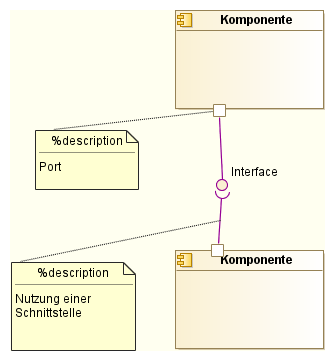
\includegraphics[scale=0.8]{uml/modelling/component.png}
    \caption{Das UML Komponentendiagramm}
    \label{fig:umlcomponentmodel}
\end{figure}

Das Komponentendiagramm modelliert im Gegensatz zum Paketdiagramm bis zu einem gewissen Grad die tatsächliche, physische Aufteilung des Systems und kann in der Architekturplanung deswegen für die Physische bzw. Verteilungssicht verwendet werden \cite[S. 223]{glasklar}\cite[S. 139]{basiswissen}. Durch die Verwendung von Interfaces ermöglicht es eine grobe und frühe Übersicht über das Zusammenspiel des zu entwickelnden Systems.

\subsection{Klassendiagramm}
Das Klassendiagramm fügt sich in die Strukturdiagramme ein und modelliert die Daten, Methoden und deren Beziehungen untereinander. Es kann als Basis für die Erstellung der Datenbanktabellen verwendet werden und übernimmt somit immer öfter die Aufgaben, welche früher dem ER Diagramm zukamen. Eine weitere Aufgabe des Klassendiagramms ist die Modellierung von Interfaces. \cite[S. 108-110]{glasklar}

\begin{figure}[H]
    \centering
    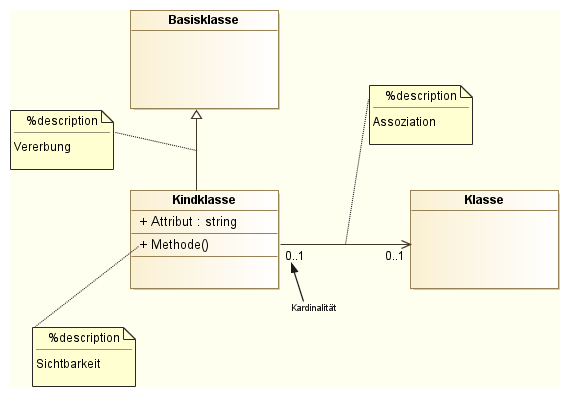
\includegraphics[scale=0.8]{uml/modelling/class.png}
    \caption{Das UML Klassendiagramm}
    \label{fig:umlclassmodel}
\end{figure}


Da die Daten und Interfaces, welche das Klassendiagramm beschreibt, auch in anderen Diagrammen referenziert werden, sind sie ein wichtiger Teil der Architekturerstellung: Interfacediagramme werden für die Beschreibung der Schnittstellen von Komponenten benötigt, Klassendiagramme werden unter Anderem in den Objektflüssen der Aktivitätsdiagramme referenziert. Außerdem lassen sich die Daten für den/die KundIn mit einem Wert beziffern, da die Vertrautheit der Daten durch Gesetze vorgeschrieben sein kann und auch ihr Verlust, Manipulation oder Diebstahl meist finanzielle Folgen nach sich zieht.


\subsection{Aktivitätsdiagramm}
Das Aktivitätsdiagramm wird in die Verhaltensmodellierung eingeteilt und erlaubt es, Abläufe des Systems zu modellieren. Es besteht aus Aktionen, Objektknoten, Kontrollelementen und Kanten, welche die Elemente untereinander verbinden \cite[S. 264]{glasklar}. Durch Objektflüsse und Swimlanes lässt sich der Austausch von Daten zwischen verschiedenen Systemen modellieren. \cite[S. 268]{glasklar}. Diese Flüsse können auch als Nachrichten im Sequenzdiagramm modelliert werden. Das Sequenzdiagramm ist aber zeitraubender zu modellieren, was dazu führt, dass die Wartung oft vernachlässigt wird \cite[S. 414]{glasklar}. \cite[S. 263-274]{glasklar}


\begin{figure}[H]
    \centering
    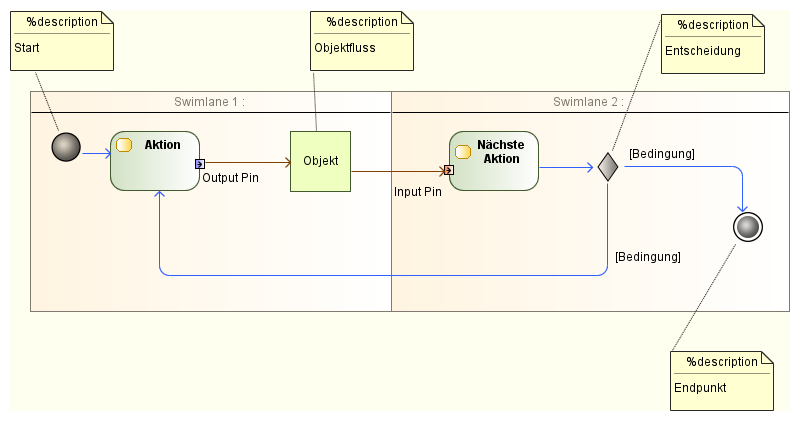
\includegraphics[scale=0.6]{uml/modelling/activity.png}
    \caption{Das UML Aktivitätsdiagramm}
    \label{fig:umlactivitymodel}
\end{figure}


Da sich das Aktivitätsdiagramm vor Allem zur Beschreibung von Businessprozessen und Usecases eignet, ist es bei der Architekturerstellung vor Allem für das Verständnis des Usecasediagrammes wichtig \cite[S. 271-272]{glasklar}. Zusätzlich helfen die modellierten Objektflüsse und Swimlanes bei der Erstellung der Komponenteninterfaces.